\documentclass[dvipdfmx]{jarticle}
\usepackage{graphicx}
\usepackage[top=30truemm,bottom=30truemm,left=25truemm,right=25truemm]{geometry}
\usepackage{listings,jvlisting}

\lstset{
  basicstyle={\ttfamily},
  identifierstyle={\small},
  commentstyle={\smallitshape},
  keywordstyle={\small\bfseries},
  ndkeywordstyle={\small},
  stringstyle={\small\ttfamily},
  frame={tb},
  breaklines=true,
  columns=[l]{fullflexible},
  numbers=left,
  xrightmargin=0zw,
  xleftmargin=3zw,
  numberstyle={\scriptsize},
  stepnumber=1,
  numbersep=1zw,
  lineskip=-0.5ex
}

\begin{document}
\begin{titlepage}
    \begin{center}
        {\huge 情報科学実験A レポート4}
        \vspace{180pt}\\
        \begin{tabular}{rl}
            氏名 & 山久保孝亮\\
            所属 & 大阪大学基礎工学部情報科学科ソフトウェア科学コース\\
            学籍番号 & 09B22084\\
            提出日 & \today\\
            担当教員 & 繁田 浩功/桝井 晃基
        \end{tabular}
    \end{center}
\end{titlepage}
\section{実験ペアの名前および学籍番号}
\begin{table}[h]
    \centering
    \begin{tabular}{|c|c|}
        \hline
        学籍番号 & 名前\\\hline\hline
        09B22083 & 安川雄輝\\\hline
    \end{tabular}
    \caption{ペアの学籍番号と名前}
\end{table}
\section{送受信回路のステート・マシンの概要図}
送受信回路のステート・マシンの概要図は以下の図1,図2のようになった.
\begin{figure}[h]
    \begin{minipage}[b]{0.45\linewidth}
      \centering
      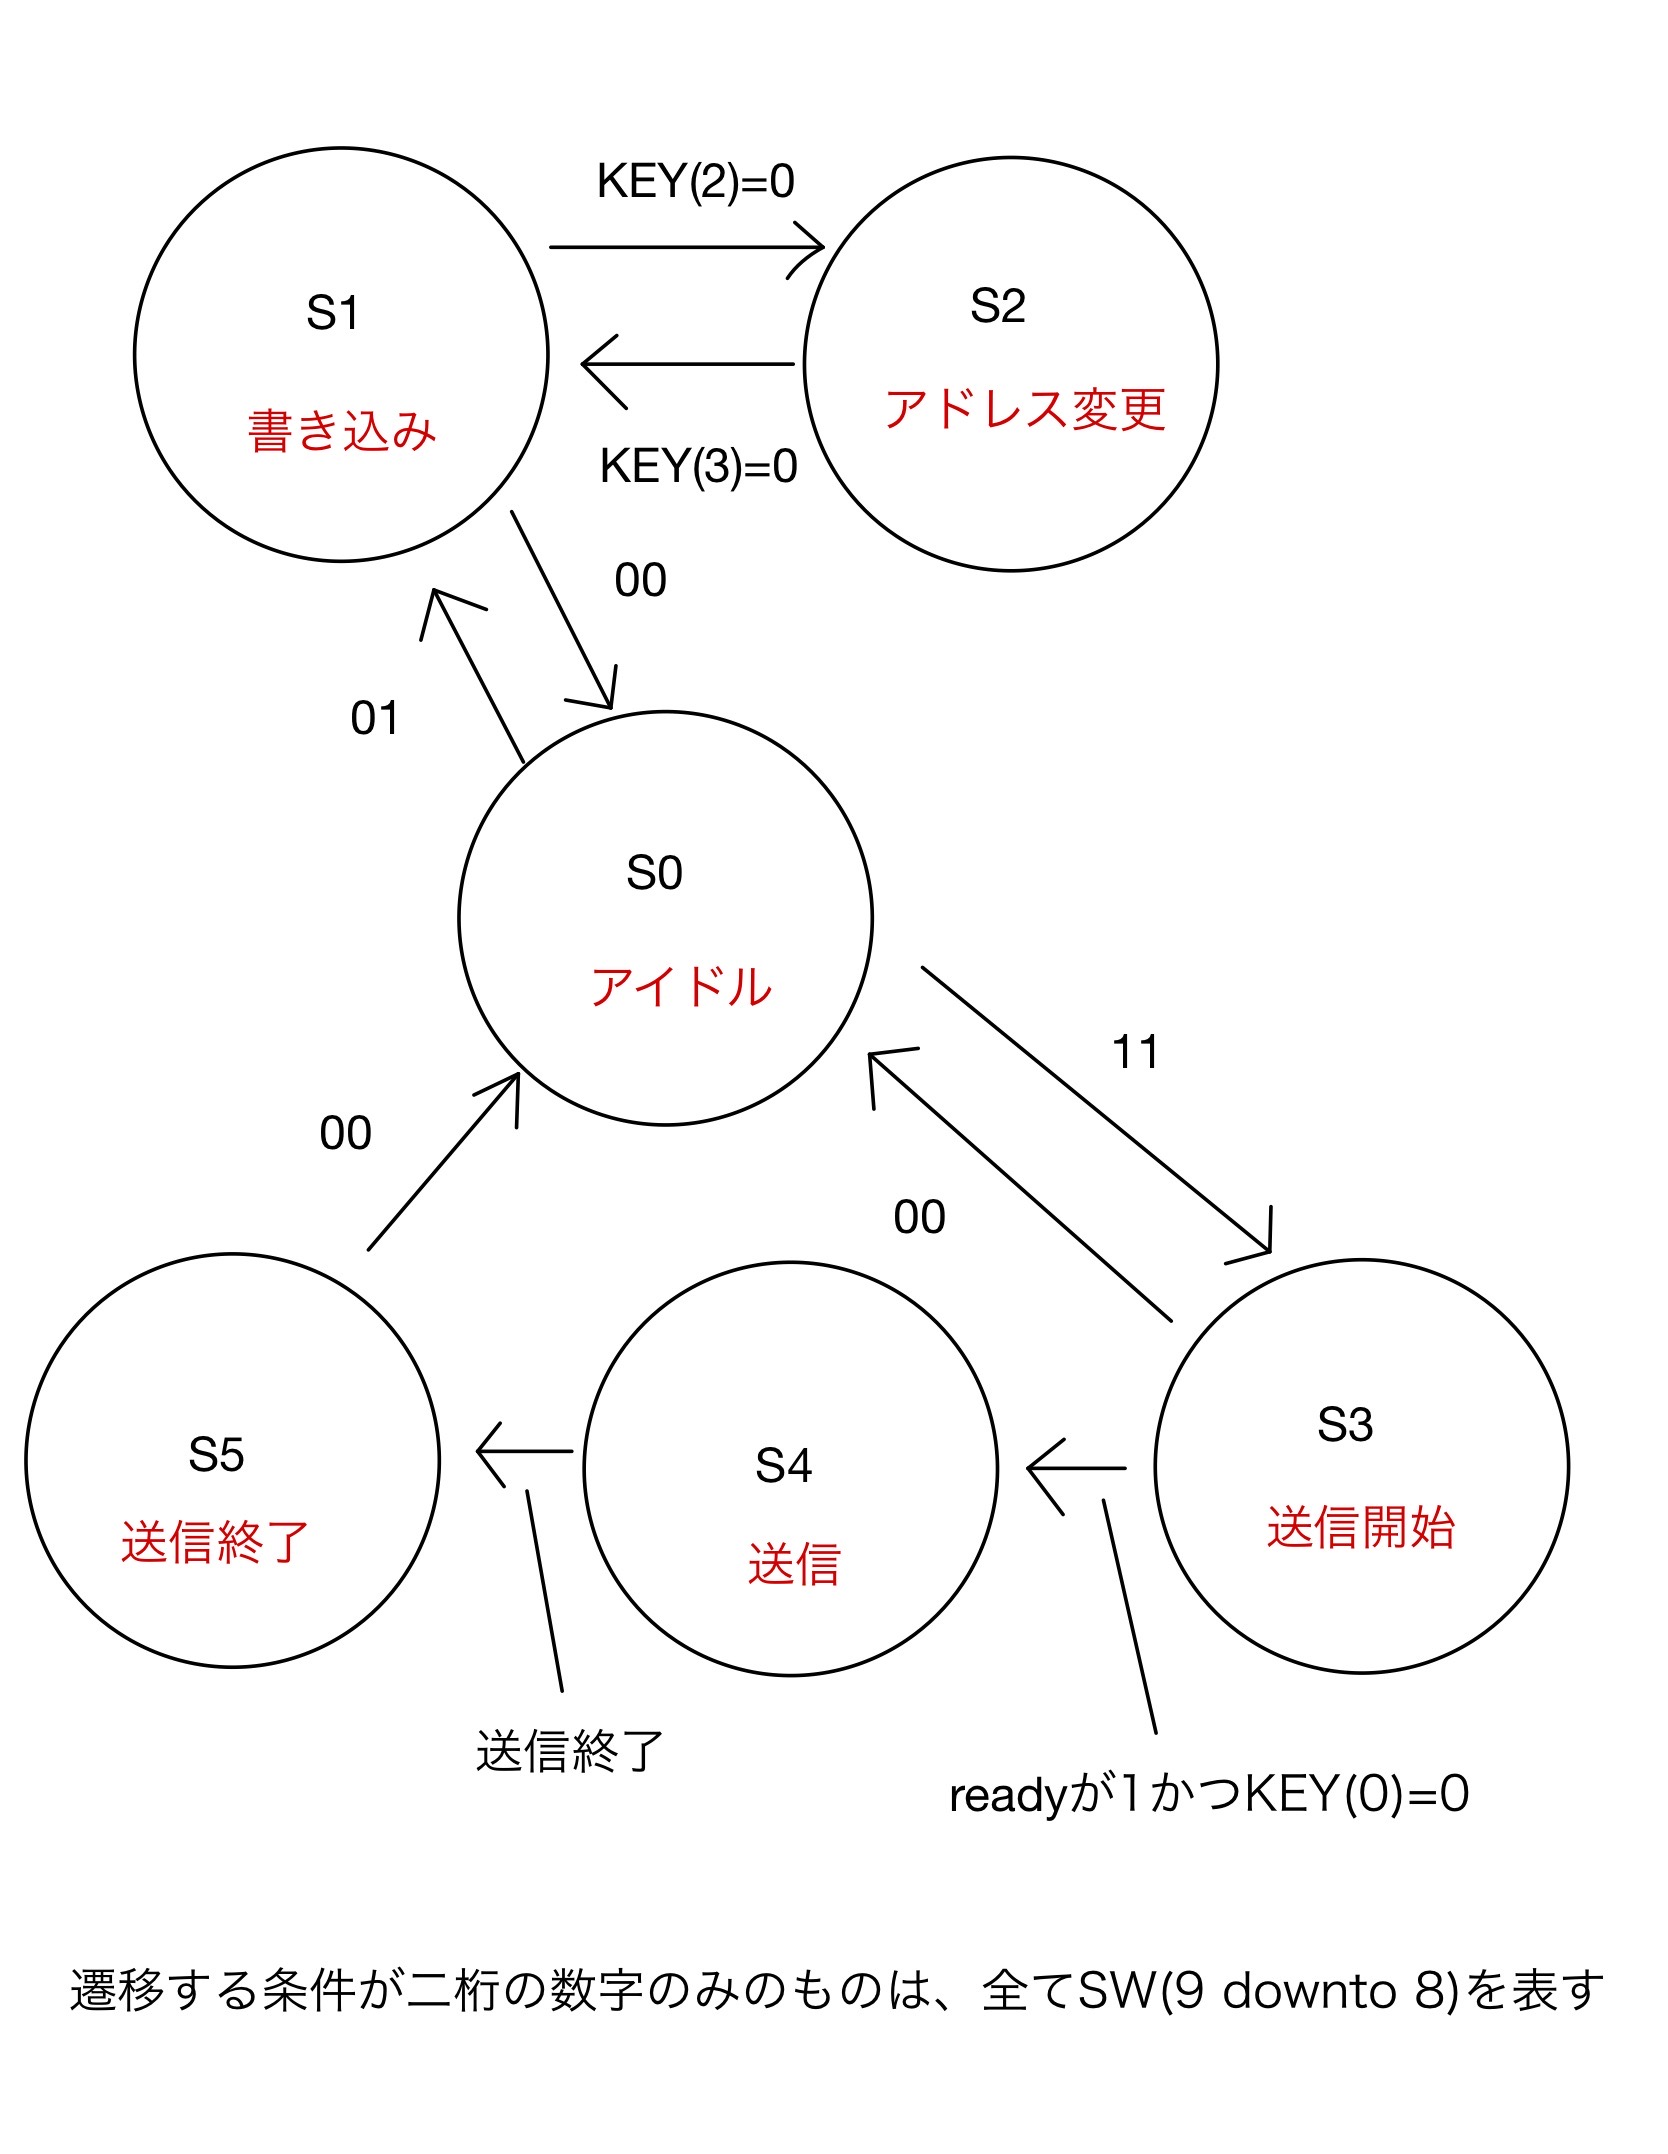
\includegraphics[keepaspectratio, scale=0.1]{state_serve.jpg}
      \caption{送信回路のステート図}
    \end{minipage}
    \begin{minipage}[b]{0.45\linewidth}
      \centering
      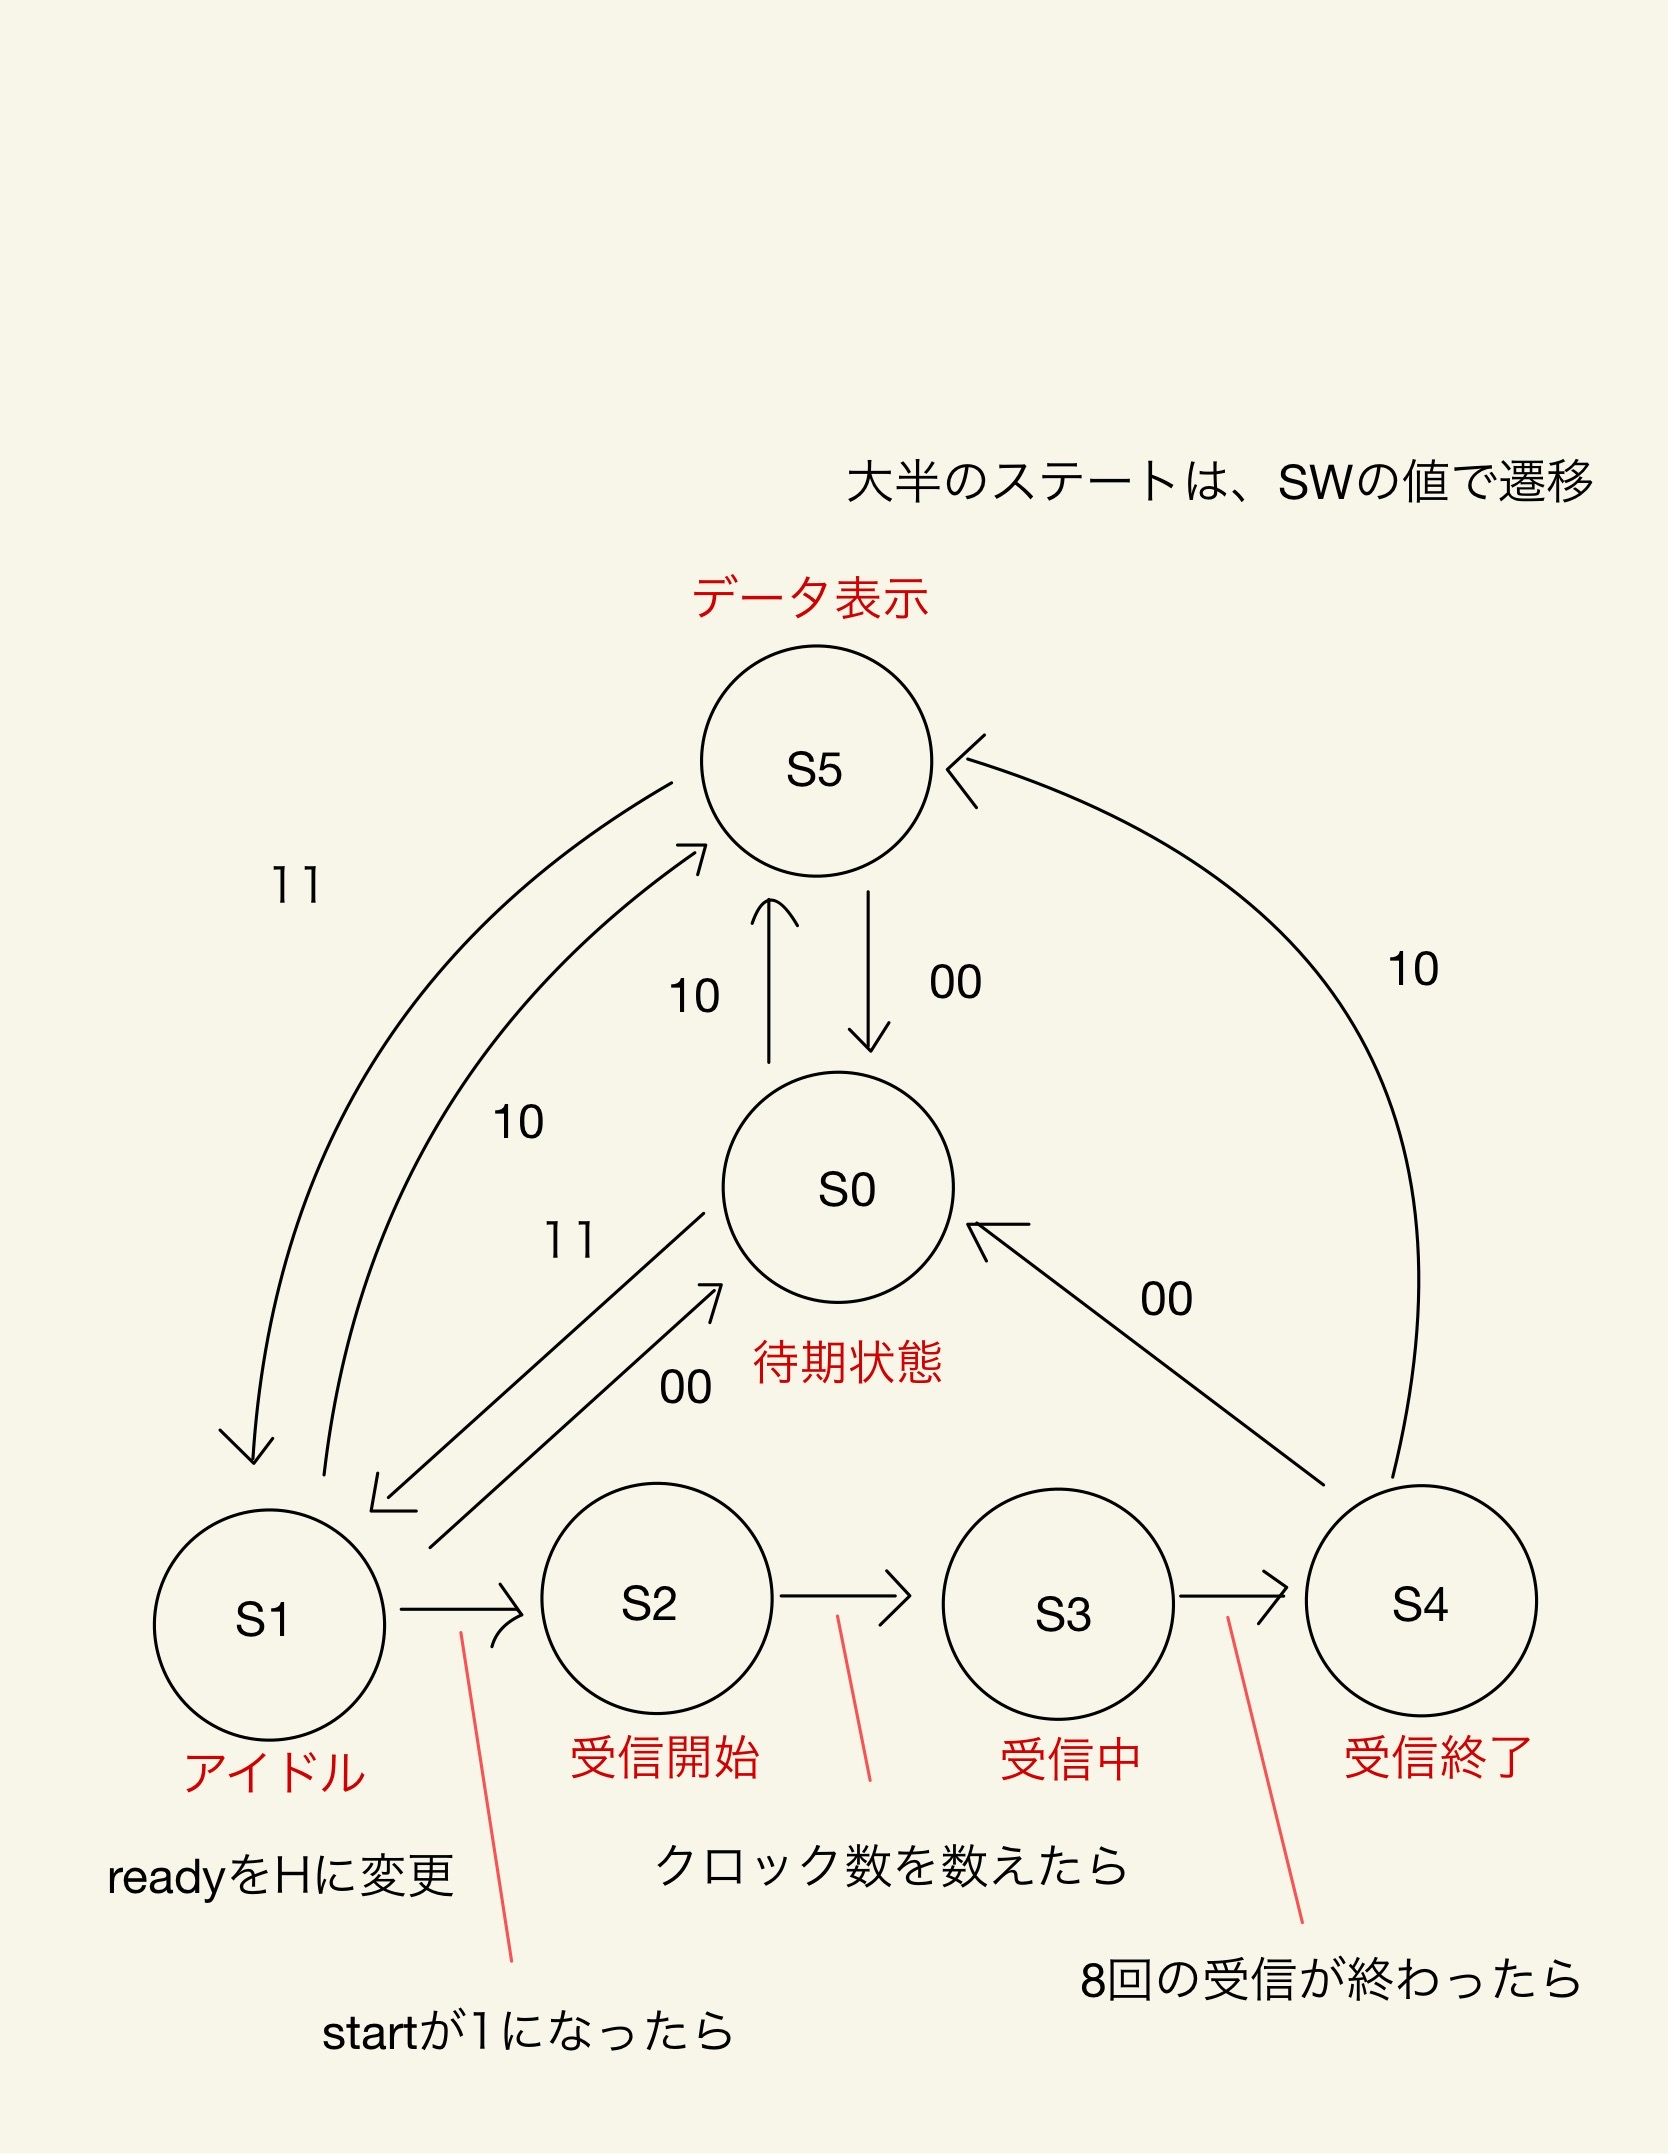
\includegraphics[keepaspectratio, scale=0.1]{state_receive.jpg}
      \caption{受信回路のステート図}
    \end{minipage}
  \end{figure}
\section{送受信回路の設計内容}
\subsection{送信回路の設計}
以下では図1のそれぞれのステートにおける処理を記述する.
\subsubsection{アイドル状態}
s0であるアイドル状態について記述する.32ビットのベクトルであるSWの8から9ビット目を参照しその値によって次の遷移先を決定する.01ならs1に遷移し,11ならs3に遷移する.
それ以外であればs0にとどまり続ける.また,s1に遷移する際にはwadrを000に,key2\_fragを0に,write\_inを0000に初期化する.
これらの変数の具体的な働きは後述する.また,このときにKEY(0)が0であるかどうかを判定し0であればkey2\_fragを1としているがこれは
テストベンチのKEYの切り替わりをステートの遷移後に計測しているとデータを書き込むのに間に合わなかったので追加した.
\subsubsection{書き込み状態}
s1である書き込み状態について記述する.KEY(0)が0になっている,即ちKEY(0)が押されるとkey2\_fragという変数が1となる.このkey2\_fragという変数はKEY(2)が押されたことを記憶しておく変数である.
そしてこのkey2\_fragが1であればkey2\_frag,KEY(3)が押されたかどうかを判定するkey3\_fragを0にしてwrite\_inに現在のdinの値を格納する.dinはram1の入力であり
一度write\_inに退避させておくことで次のアドレス変更状態にいる際にデータが変更されても書き込むデータ自体はKEY(2)を押したタイミングでのデータであり続けるからである.そしてその後
s2に遷移する.また,s0の時と同様にSWの8から9ビットが00であればs0に遷移し,以上どの分岐にも当てはまらない場合にはs1にとどまり続ける.

\subsubsection{アドレス変更状態}
s2であるアドレス変更状態について記述する.KEY(2)やKEY(3)が押されるとそれぞれのfragの変数が1となる.
key3\_fragが1であるかどうかを判定し,1であればkey3\_fragを0にしwadrを1だけ増やす.これにより加算される前のwadrの
値に対応するデータの値が確定する.そして分岐に当てはまらなければs2にとどまり続ける.
\subsubsection{送信開始状態}
s3である送信開始について記述する.SWの8から9ビットが00であればs0に遷移する.次に受信側が送ってくるreadyが1であるかどうかを判定する.
readyが1でなければs3にとどまり続け以降の判定は行わない.readyが1のときはKEY(0)が0かどうかを判定する.0であればradrを000に,countを1に初期化してs4に遷移する.
\subsubsection{送信状態}
s4である送信状態について記述する.ここではまずクロック生成をしてそのクロックの周期を受信側に伝える処理を行う.受信側に伝え終わったときに1となる変数finishが0であるかどうかを判定し,
0であればenableを1にしてクロックの生成を開始する.その後生成したclock\_txが立ち上りでなければstartを1にして受信側にクロック生成が開始されたことを伝える.また,このとき送信時に使用するクロックの周期をそろえるためにcount\_clockというカウンタを用意し,
送信側のクロック周期何回分が生成クロックの周期に対応するのか計測しておく.これは送信側と受信側の情報のやり取りをするタイミングをそろえるためである.
clock\_txが立ち上がりであればstart,enableを0にして周期を伝えることとクロック生成終了する.また,finshを1にして送信状態の次の処理を実行する.ところで,生成クロックの立ち上がりを測定することはclock\_tx\_lastという直前の生成クロックの値を格納する変数を用意しておき,
現在の生成クロックの値が1で,直前の値が0のときという条件分岐を作って実現した.
\\そのあとすぐにデータの送信を開始する.送信したデータの個数を表すcount\_sendという変数が8かどうかを判定することで7以下である場合は同じ処理が繰り返されるようにした.7以下である場合は送信側のクロックが何回立ち上がったかを記憶するclockという変数が先ほど計測したcount\_clockから1引いた値と同じになったタイミングで
データを送信する.今回送信するデータと実機の7セグメントデコーダの対応は以下の通りである.
\clearpage
\begin{table}[h]
  \centering
  \begin{tabular}{|c|c|}
    \hline
    7セグメントデコーダの番号 & 送信するデータ\\
    \hline\hline
    HEX0 & 何も送信しないので常に0を表示\\\hline
    HEX1 & 送信するデータ\\\hline
    HEX2 & 何も送信しないので常に0を表示\\\hline
    HEX3 & 送信するデータのアドレス\\\hline
    HEX4 & 何も送信しないので常に0を表示\\\hline
    HEX5 & GPIO\_1(5)の内容 \\\hline
    \hline
  \end{tabular}
  \caption{7セグメントデコーダの送信するデータの対応表}
\end{table}
\subsubsection{送信終了状態}
s5である送信終了状態について記述する.SWの8から9ビットが00であればradr,clk\_tx\_last,count,count\_send,count\_clkを初期化してs0に遷移する.それ以外の時はs5にとどまり続ける.

\subsection{受信回路の設計}
以下では図2のそれぞれのステートにおける処理を記述する.
\subsubsection{待機状態}
s0である待機状態ではSWの8から9ビットの値によってstateを遷移させる.11のときはs1に遷移し10のときはs5に遷移する.
\subsubsection{アイドル状態}
s1であるアイドル状態ではready信号を1にして送信側のstartが1になるのを待つ状態である.
\subsubsection{受信開始状態}
s2である受信開始状態では
\subsubsection{受信中状態}
s3である受信中状態では
\subsubsection{受信終了状態}
s4である受信終了状態では
\subsubsection{データ表示状態}
s5であるデータ表示状態では
\section{テストベンチによる動作確認内容・結果}
テストベンチは配布されていたものをそのまま利用した.
\subsection{送信回路の動作結果}
\subsubsection{データ書き込みの動作}
以下の図はデータ書き込みを行う際の波形である.以下でその詳細を記述する.
\begin{figure}[h]
  \centering
  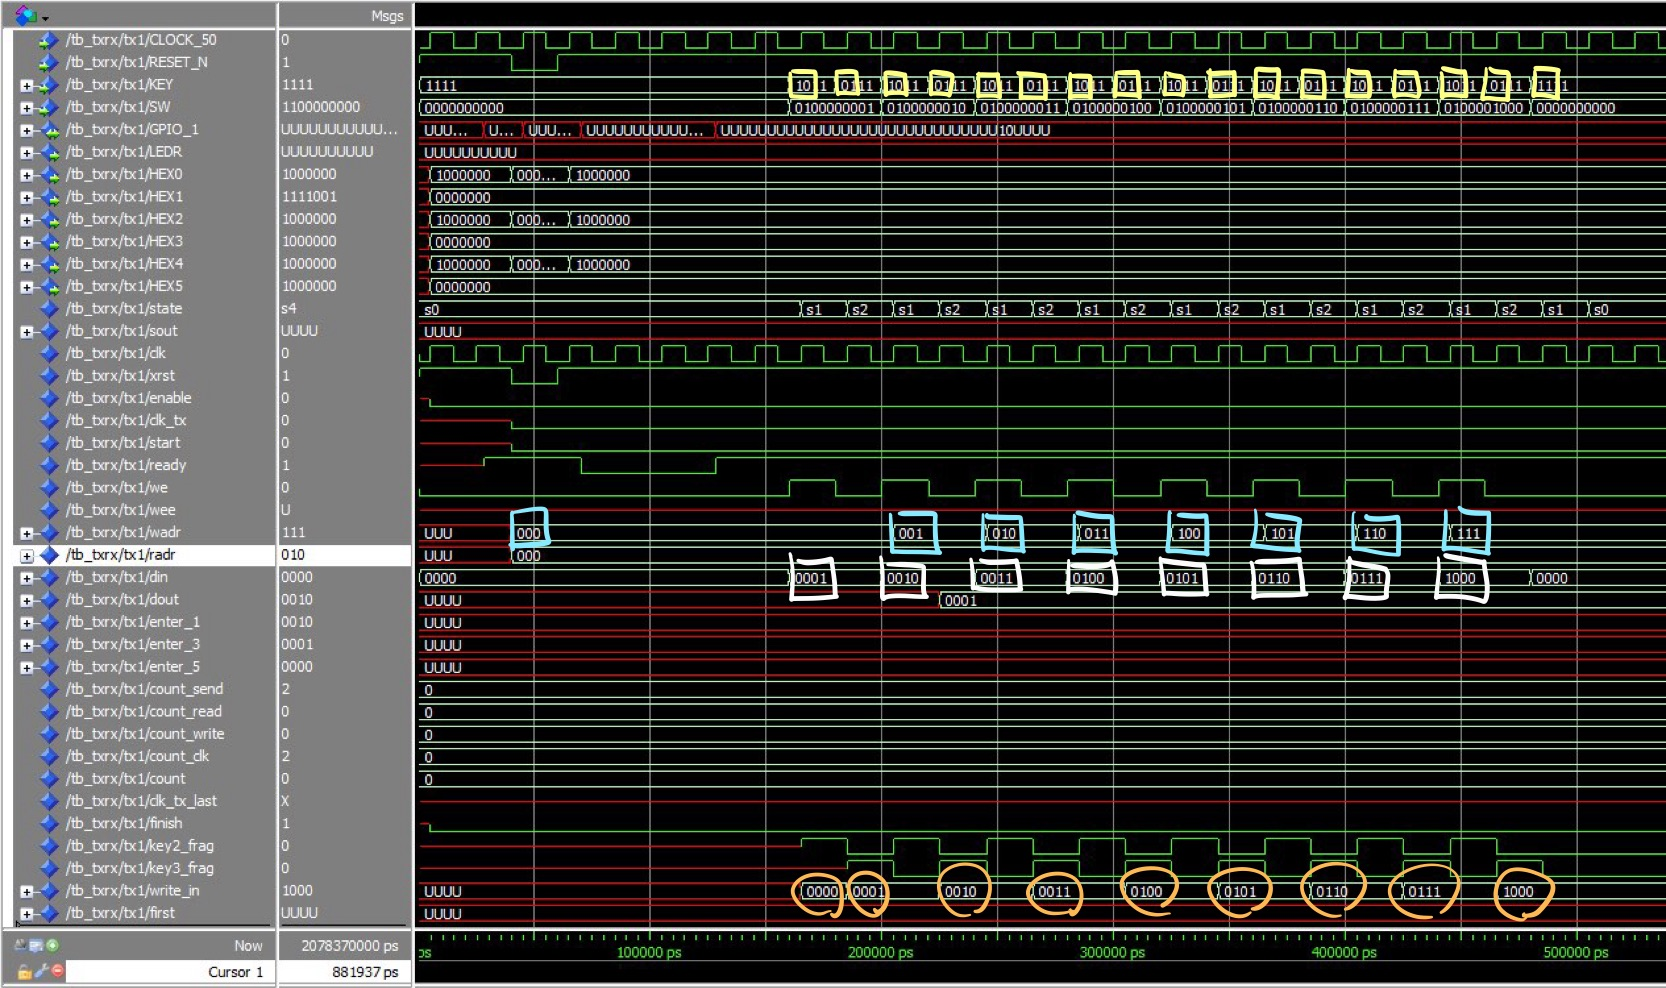
\includegraphics[width=12cm]{wave_write.jpg}
  \caption{データ書き込みの際の波形}
\end{figure}
白く囲まれた一番上の段の一番左のビットであるKEY(3)が0になったときに状態がs2に遷移し,直前の状態であるs1のときのdinの値がwrite\_inにコピーされていることがわかる.また,
オレンジで囲った処理によりKEY(2)が変更されると状態がs1へ遷移し,wadrの値が1増やされていることがわかる.
これらの操作は合計で8回行われているため8回分のデータを書き込むことができている.
\subsubsection{データ送信の動作}
以下の図はデータ送信時の波形である.以下でその詳細について述べる.
\begin{figure}[h]
  \centering
  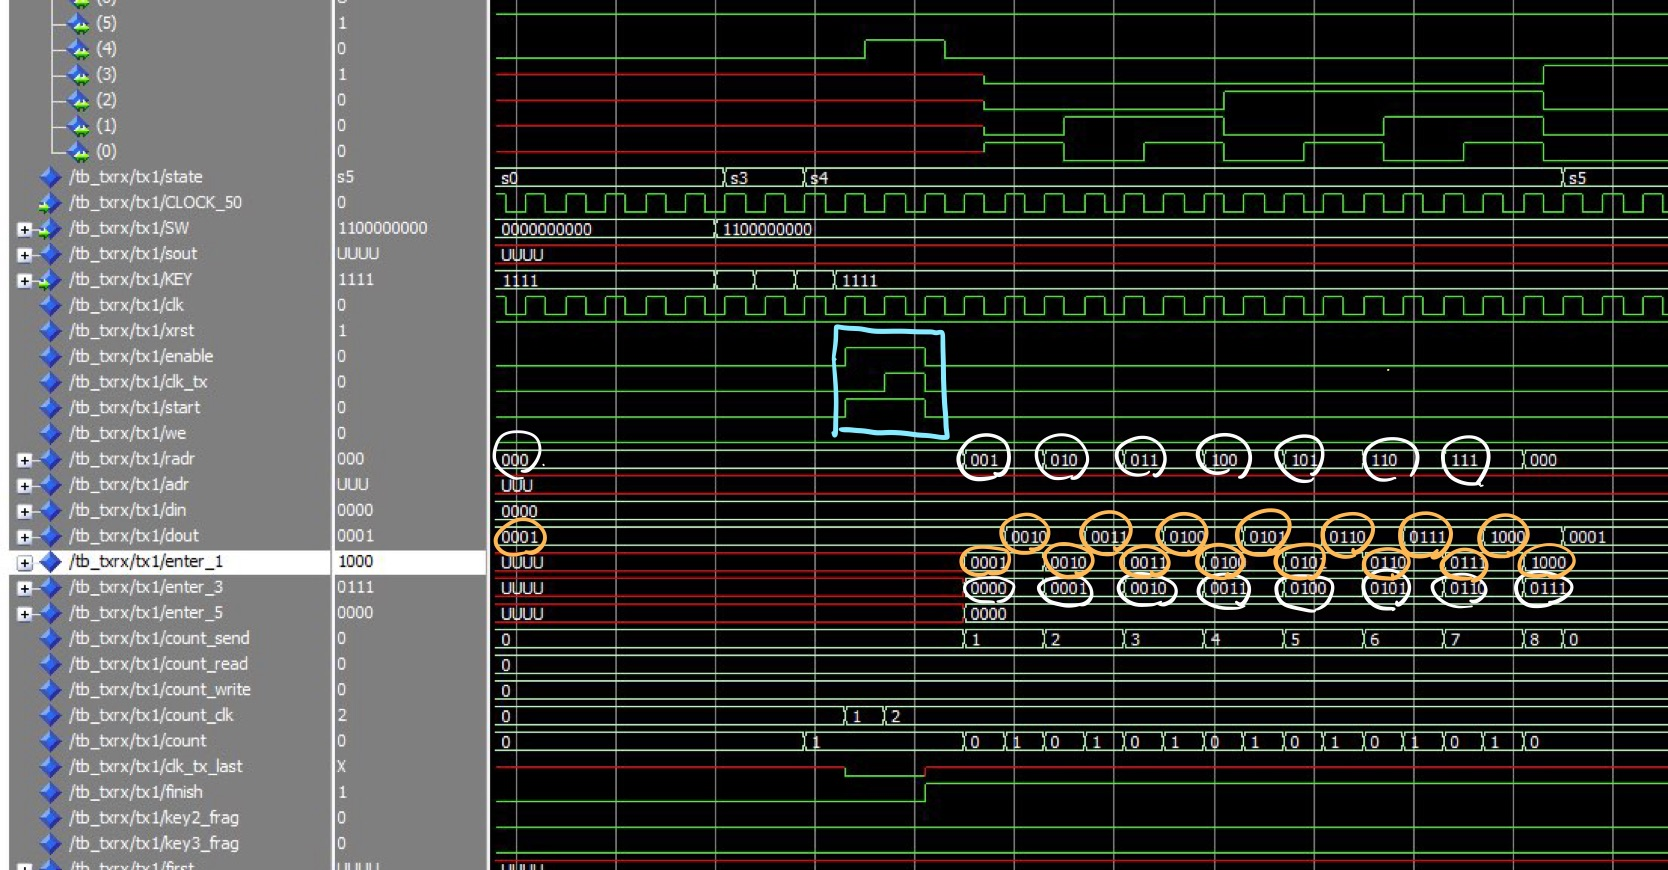
\includegraphics[width=12cm]{wave_send.jpg}
  \caption{データ送信の際の波形}
\end{figure}
水色で囲んだ部分から状態がs4に遷移した後にenableとstartが同じタイミング1となっている.また,この期間はclock\_txの一周期分となっているため正しい.
また白色に囲んだ部分から一つ前のradrの値がenter\_3に,オレンジに囲んだ部分から一つ前のdoutの値がenter\_1に入っている.これは先ほど書き込んだデータを同じアドレスで出力できている.
\subsection{受信回路の動作結果}
\section{非同期通信回路作成における注意点などの考察}
今回の課題を通して非同期通信回路を作成するにあたって注意しなければならない点は以下の2点であると考えた.
\begin{enumerate}
  \item クロックを生成し終えてからデータを送信するまでのタイミングを合わせること.
  \item アドレスが000に戻ったときに000に格納されているデータが変化してしまう.
\end{enumerate}
以下でその詳細について述べる.
\begin{enumerate}
  \item 今回の実験の仕様から,KEY(2)が押されるとSWの下位4ビットの値の送信を開始する状態に遷移し,そのあとKEY(3)を押すとクロックを生成する.そして最後にデータを送信するが,
クロック生成を終えてからデータを送信する間を制御するボタンが設定されていない.今回の課題では設計内容で記述した通りクロック生成が終了した後すぐにデータを送信したが,この部分は送信側と受信側できちんと
あらかじめ決めておく必要がある.
  \item RAMにデータを書き込む際は書き込むためのアドレスの値が変化したとき,最後に入力に入っていた値が格納される.即ちアドレスが変更された瞬間に変更される前のアドレスに格納されるデータが確定し,現在のアドレスが指すRAMの内容は常に変動しているということである.
今回のアドレスは3ビットのベクトルを1ずつ増やしていくことでアドレスを実現したが,111の状態で1を加算すると000に戻ってしまっていた.したがって,最初に000のアドレスにデータを格納した後に111までデータを格納すると,アドレスが000まで戻ってしまうため000のアドレスに格納されている値が変化してしまう.
\end{enumerate}
\section{教員・TAによる動作確認時刻}
1月25日18時15分
\end{document}